In this section we will detail the design of our tool, the algorithm and its parameters.
\subsection{Algorithm}
\subsubsection{Input and output}
The algorithm accepts a matrix X = n x k of input data, and a vector Y = 1 x k of expected data. It will evolve expressions that result, when evaluated on X, in an 1 x k vector Y' that approximates Y. N is the number of features, or parameters, the expression can use. We do not know in advance if all features are needed, which makes the problem statement even harder.
K is the number of datapoints. The algorithm makes no assumptions on the domain or range of the expressions or data set. While domain specific knowledge can be of great value, in real world situations such data is not always known. We aim to make a tool that operates under this uncertainty.
\subsubsection{Control flow}
Figure \ref{fig:controlflow} gives a high level overview of the tool's control flow.
\begin{figure}
\begin{tikzpicture}[node distance=1.5cm, every node/.style={font=\footnotesize}]
\node (start) [startstop] {Start};
\node (phase) [decision, below of=start, yshift=-0.5cm] {Phase $<$ Phases};
\node (init) [process, below of=phase, yshift=-1cm] {0.0 Initialize};
\node (gen) [process, right of=init, xshift=4cm] {0.1 Generate random expression tree};
\node (while) [decision, below of=init, yshift=-1.5cm, align=center] {1. \\ Generation \\ $<$ \\ Generations }; % stopcondition?
\node (eval) [process, below of=while, yshift=-1.5cm] {2. Evaluate Population};
\node (select) [process, below of=eval] {3. Select};
\node (evolve) [process, below of=select] {4. Evolve};
\node (mutate) [process, right of=evolve, xshift=4cm, yshift = + 0.75 cm] {4.1 Mutate};
\node (crossover) [process, below of=mutate ] {4.2 Crossover};
\node (update) [process, below of=evolve] {5. Update Population};
\node (archive) [process, right of=while, xshift=4cm] {0.2 Archive};
\node (external) [process, right of=archive, xshift=4cm] {0.3 External process};
\node (optimizea) [process, below of=archive] {6.1 Optimize};
\node (optimizet) [process, below of=update] {6.2 Optimize};

\draw [arrow] (start) -- (phase);
\draw [arrow] (phase) -- node[anchor=east]{yes}(init);
\draw [arrow] (init) -- (while);
\draw [arrow] (while) -- node[anchor=east]{yes}(eval);
\draw [arrow] (while) -- node[anchor=south]{no}(archive);
%\draw [arrow] (archive) -- (phase);
\draw [arrow] (eval) -- (select);
\draw [arrow] (select) -- (evolve);
\draw [arrow] (evolve) -- (mutate);
\draw [arrow] (mutate) -- (evolve);
\draw [arrow] (evolve) -- (crossover);
\draw [arrow] (crossover) -- (evolve);
\draw [arrow] (evolve) -- (update);
\draw [dashed, ->] (gen) -- node[anchor=south]{seeds}(init);
\draw [dashed, ->] (archive) -- node[anchor=south]{seeds}(init);
\draw [dashed, <->] (update) -- node[anchor=east]{optional}(optimizet);
\draw [dashed, <->] (archive) -- node[anchor=east]{optional}(optimizea);
\draw [dashed, <->] (external) -- node[anchor=south]{optional}(archive);
\draw [arrow] (archive)-- +(2,0) |- (phase) node[near start,sloped,above] {};

\draw [arrow] (update)-- +(-2,0) |- (while) node[near start,sloped,above] {};
\end{tikzpicture}
\caption{CSRM control flow.}
\label{fig:controlflow}
\end{figure}
In the following sections we will discuss each of the stages and discuss the trade-offs made in our design.
\subsubsection{Entities}
We will describe briefly the important entities in our design. In Figure \ref{fig:uml} the architecture of our tool is shown. Functionality such as IO, statistics and plotting is left out here for clarity. The interested reader is referred to the source code documentation.
\paragraph{Algorithm}
The algorithm hierarchy extends each instance with new behavior, only overriding those functions needed. Code reuse is maximized here by the usage of hook functions, which in the superclasses result in a noop operation. An example of this is the evolve function, by and large the most complex function of the algorithm. By using hooks such as \textit{requireMutation()} this function can remain in the superclass, and the subclass need only implement the hook.
\paragraph{Tree}
The Tree and Node classes represent the main data structures of CSRM's population. The Tree is comprised of Node objects, each of which holds an optional constant weight. Leaves are either features or constants.
In \ref{subsectree} we go in depth into the design choices made for this representation.
The Tree class holds a few utility functions, for example to create trees from an expression using a parser in the tool module.
Functionality needed by the mutation and crossover operators is present here as well. Of note are both construction functions, which allow for efficient generation of random trees. In section \ref{subsubinvalidexpressions} we will cover the problem these functions solve.

\paragraph{Optimizer}
CSRM provides an interface to continuous optimizers. In section \ref{secconstopt} we will go deeper into the specific algorithms used. The population data structure is shared between the subclasses. The instances in the population can be subclassed if specific functionality is needed by an optimizer. This approach allows us to reuse a large part of the code between algorithms. For convenience a stub optimizer is added. The optimization algorithms share configuration parameters, and encapsulate those that are distinct to their specific nature.
% Distributed aspect in distributed paper
\begin{figure}
    \centering
    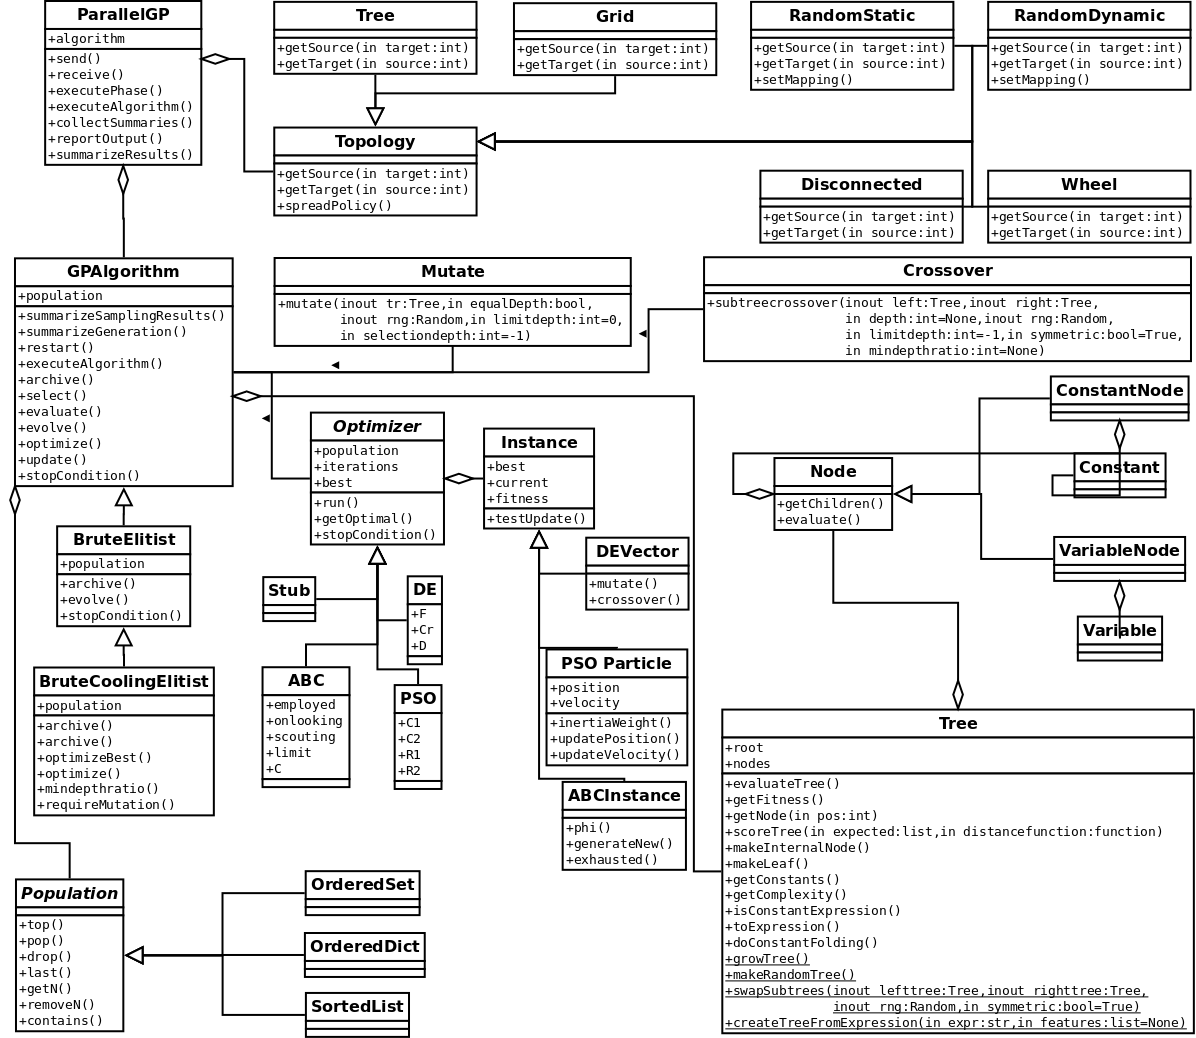
\includegraphics[width=\textwidth,height=\textheight,keepaspectratio]{figures/umldistributed.png}
    \caption{UML of CSRM.}
    \label{fig:uml}
\end{figure}


\subsubsection{Implementation}
Our tool is implemented in Python. The language offers portability, access to rich libraries and fast development cycles. The disadvantages are speed and memory usage compared with compiled languages (e.g. C++) or newer scripting languages (e.g Julia). % ref julia.
Furthermore, Python's usage of a global interpreter lock makes shared memory parallelism not feasible. Distributed programming is possible using MPI.

\subsection{Fitness}
In this work we interpret optimization as a fitness minimization process. In the following we will discuss the fitness function and its behavior.
\subsubsection{Distance function}
The goal of the algorithm is to find f' such that
\[Y = f(X)\]
\[Y' = f'(X)\]
\[dist(Y, Y') = e\]
results in e minimal. F is the process we wish to model or approximate with f'.\\
Not all distance functions are equally well suited for this purpose. A simple root mean squared error (RMSE) function has the issue of scale, the range of this function is [0, +$\infty$), which makes comparison problematic, especially if we want to combine it with other objective functions. A simple linear weighted sum requires that all terms use the same scale.
Normalization of RMSE is an option, however there is no single recommended approach to obtain this NRMSE. \\
In this work we use a distance function based on the Pearson Correlation Coefficient. Specifically, we define
\[
dist_p(Y, Y') = 1 - \vert r \vert
\]
with
\[
r = \frac{\sum_{i=0}^{n}{(y_i-E[Y])*(y'_i-E[Y'])}}{\sqrt{\sum_{j=0}^{n}{(y_j-E[Y])^2}*\sum_{k=0}^{n}{(y'_k-E[Y'])^2}}}
\]
R has a range of [-1, 1] where 1, -1 indicate linear and negative linear correlation respectively, and 0 indicates no correlation.
This function has a range [0,1] which facilitates comparison across domains and allows combining it with other objective functions.
The function reflects the aim of the algorithm. We not only want to assign a good (i.e. minimal) fitness value to a model that has a minimal distance, we also want to consider linearity between Y an Y'. The use of the Pearson correlation coefficient as a fitness measure is not new, a variant of this approach is used in \citep{pearson}.

\subsubsection{Diversity}\label{subsubdiversity}
Diversity, the concept of maintaining semantically different specimens, is an important aspect in metaheuristics. Concepts such as niching and partitioning are often used to promote this behavior, amongst other reasons to prevent premature convergence or even to enable multimodality.
Our tool uses a simple measure that approximates the more advanced techniques stated above. It should be clear that for any combination of input and output data, there are is huge set of expressions with identical fitness values. Such expressions can lead to premature convergence where a subset of the fittest expressions all have the same fitness value without introducing new information. Those expressions approximate the same local optimum. Our tool will aim to prevent retaining expressions that have identical fitness values.
%Some metaheuristics \cite{DE} allow replacement of solutions with identical fitness values as it can help avoid local minima.
There are disadvantages to this approach, if the fitness function has a zero gradient surface allowing replacement based on equal fitness value can help the optimizer to traverse such an area.

\subsubsection{Predictive behavior}
The algorithm evaluates expressions based on training data $X_t \subset X$. $X_t$ is an n x (rk) matrix sampled from the original input matrix X, with $r \in ] 0,1 [$.
R is the sampling ratio, the ratio between training and validation data.
After completion of the algorithm the population is ordered based on minimized fitness values calculated on the training data.
In real world applications practitioners are also interested in the predictive qualities of the generated expression. In other words, how well do the expressions score on unknown data? In the final evaluation we score each expression on the full data to obtain this measure.
While this gives us some information on how good an expression is on the full data set, we are also interested in how the convergence rate corresponds to the final fitness value on the full data.
If we add 10 more generations, or increase the population by a factor 1.5, what do we gain or lose in predictive quality of the expressions?
To define this we use a correlation measure between the fitness values using the training data and those of the full data.
This measure quantifies the predictive value of the final results.
Finally, we calculate a correlation trend between the training fitness values at the end of each phase, and the final fitness values calculated on the full data. This trend describes the convergence process of the algorithm over time, specifically directed at the predictive value of the solutions found. It is important to note that the entire final population is considered in these calculations, not only the best. While ideal, there is no guarantee that the expression that has the lowest fitness value on the training data will score best on the full data set. Using this correlation measure we can estimate how the convergence rate on the unknown data evolves over time. This measure then also serves as an indicator for overfitting.

\subsubsection{Convergence limit}
As a stopcondition our tool uses a preset number of iterations. The user specifies the number of generations (g) and phases (r), and the algorithm will at most execute g x r iterations. Convergence stalling is implemented by keeping track of the number of successful operations (mutation or crossover). If this value crosses a threshold value convergence has stalled and the algorithm is terminated. An alternative stopcondition is a minimum quality or fitness that should be achieved. This is very hard to estimate. The topology of the fitness function is highly problem dependent. The 'hardness' \citep{GPHardness} of the problem will determine the convergence rate. Given that the desired solution is not known, it is impossible for a practitioner to know in advance how much time the algorithm will need in order to obtain the desired quality of solution. It is even possible that the algorithm converges to a suboptimal value with a fitness value strictly greater than the desired value. For these reasons we opted for a simple but robust stopping condition.


\subsection{Initialization}
Initialization is done using the 'full' method \cite{GP}. The algorithm has a parameter initial depth, each new expression in the population is created using that depth. Unless the maximum depth is equal to the initial depth, the algorithm will quickly vary in depth, evolving an optimal depth.

\subsubsection{Invalid expressions}\label{subsubinvalidexpressions}
Generating a random expression is done by generating random subtrees and merging them. An important observation here is that randomly generated expressions can be invalid for their domain. The ubiquitous example here is division by zero. Several approaches to solve this problem exist. One can define 'safe' variants of the functions, in case of division by zero, returning a predefined value that will still result in a valid tree. The downside to this approach is that the division function's semantics are altered. A practitioner, given an expression, would have to know that some functions are no longer corresponding entirely to their mathematical equivalents, and what 'safe' values the implementation uses.
The other option is assigning maximum fitness to an invalid expression. While simple, this approach needs a careful implementation. From a practical standpoint wrapping functions in exception handling code will quickly deteriorate performance.
Our approach is a domain check for each function, and communicating by return value if the domain check failed thereby avoiding exceptions.

\paragraph{Invalidity probability}
We define the probability that a randomly generated tree of depth d, with n possible features, k possible base functions, and j data points as q. With more complex problems d will have to be increased. GP is also susceptible to bloat \cite{GPBloat}, increasing d even further. This issue will affect generation of subtrees in mutation. With more datapoints the probability of at least one leading to an invalid evaluation will increase. An increase in d will lead to an exponential increase in the number of nodes in the tree. A node can be either a basefunction or a leaf (feature or constant). For each additional node the probability q increases. We can conclude that q, while irrelevant for small problems and depths, becomes a major constraint for larger problem statements.

\paragraph{Bottom up versus top down}
There are two methods to generate a tree based expression : bottom up and top down. The top down approach is conceptually simpler, we select a random node and add randomly selected child nodes until the depth constraint in satisfied. The problem with this approach is that the expression can only be evaluated at completion, early detection of an invalid subtree is impossible.
In contrast in a bottom up construction we generate small subtrees, evaluate them and if and only if valid merge them into a larger tree. This allows for early detection of invalid expressions. A downside of this approach is the repeated evaluation of the subtrees, which can be mitigated by caching the result of the subtree.

\paragraph{Disallowing invalid expressions in initialization}
We can generate random expressions and let the evolution stage of the algorithm filter them out based on their fitness value, or we can enforce the constraint that no invalid expressions are introduced. The last option is computationally more expensive at first sight, since the algorithm is capable by definition of eliminating unfit expressions from the population.
This can lead to unwanted behavior in the algorithm itself. For high q values we can have a significant part of the population that is at any one time invalid. This can lead to premature convergence, similar to a scenario where the population is artificially small or dominated by a set of highly fit individuals. Another observation to make is that the algorithm will waste operations (mutation, crossover) on expressions that are improbable to contribute to a good solution.
While more expensive computationally, we therefore prohibit the generation of invalid expressions in the initialization.

\subsection{Evaluation and cost}
Expression evaluation requires a tree traversal for each datapoint. In order to compare optimization algorithms across implementations practitioners can use as a measure the number of evaluations required to reach a certain fitness level. If this measure is used, one should take into account that not all evaluations are equal. With the trees varying in depth and density the evaluation cost varies significantly. Furthermore, evaluating "1 + 2" is computationally far less expensive than "log(3, 4)". A simple count of evaluation functions executed does not really reflect the true computation cost, especially when we consider the variable depth of the trees. Increasing the depth leads to an exponential increase in the number of nodes, and thus in the evaluation cost.
Our tool uses a complexity measure that takes into account the density of the tree and which functions are used. A tree comprised of complex functions will score higher in cost than a corresponding tree using simple multiplications and additions. Although this is an option, we do not use this measure in the objective function. We would like to observe the effect of this cost, but not have it directly influence the algorithm. There is no direct link between more complex functions and an optimal solution. In certain domains the argument can be made that more complex functions are more likely to lead to overfitting, or more likely to lead to invalid trees due to a smaller domain.

\subsection{Evolution}
In the evolution stage we apply two operators on (a selection of) the population. The operators are configured to constrain the depth of the modified trees, enforcing the maximum depth parameter.
We trace the application of the operators during the execution using an effectiveness measure. Each time an operator application is able to lower the fitness of a tree, this measure increases. Using this measure we can gain insight when and how certain optimizations and modifications work inside the algorithm instead of simply observing the algorithm as a black box.
 \begin{figure}
    \centering
    \begin{subfigure}{0.5\textwidth}
    \centering
        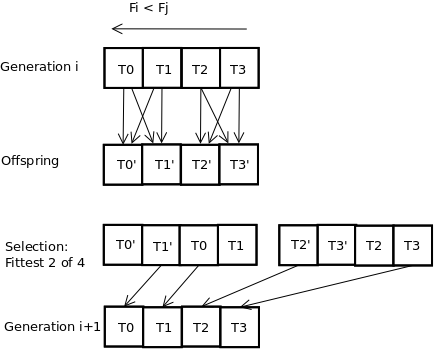
\includegraphics[width=0.8\linewidth]{figures/pairwisecrossover.png}
        \caption{Pairwise crossover.}
    \end{subfigure}
    \begin{subfigure}{0.5\textwidth}
    \centering
        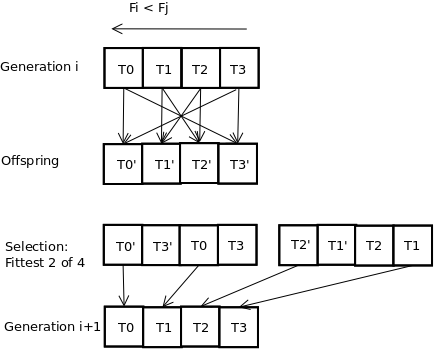
\includegraphics[width=0.8\linewidth]{figures/randomcrossover.png}
        \caption{Random crossover.}
    \end{subfigure}
    \caption{Selection procedures applied by crossover.}
    \label{fig:crossoverselection}
\end{figure}

 \begin{figure}
    \begin{subfigure}{0.5\textwidth}
        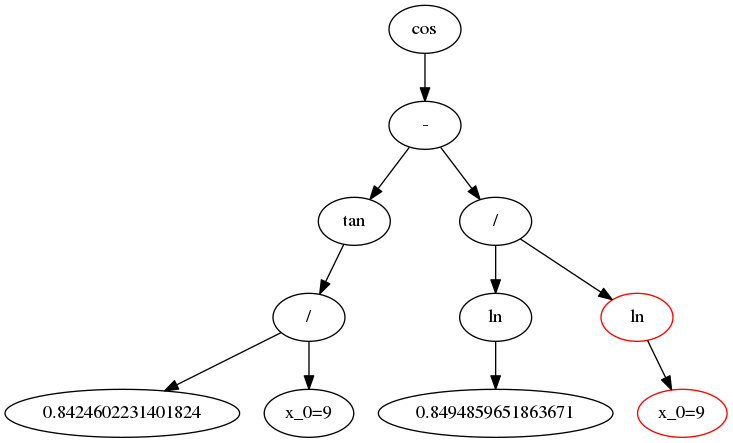
\includegraphics[width=0.8\linewidth]{figures/leftbefore.png}
        \caption{A before crossover.}
    \end{subfigure}
    \begin{subfigure}{0.5\textwidth}
        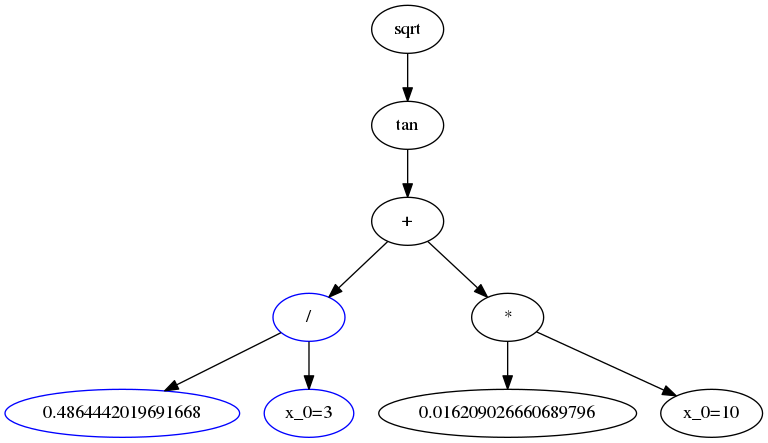
\includegraphics[width=0.8\linewidth]{figures/rightbefore.png}
        \caption{B before crossover.}
    \end{subfigure}
        \begin{subfigure}{0.5\textwidth}
        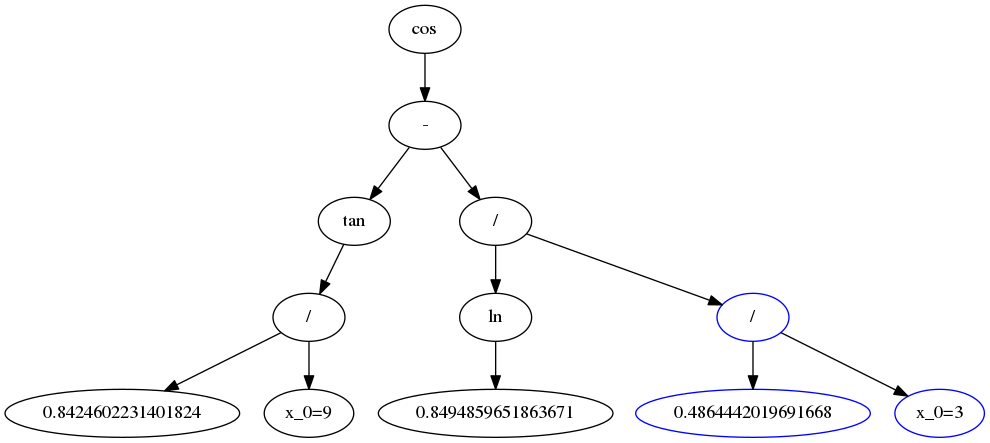
\includegraphics[width=0.8\linewidth]{figures/leftafter.png}
        \caption{A after crossover.}
    \end{subfigure}
    \begin{subfigure}{0.5\textwidth}
        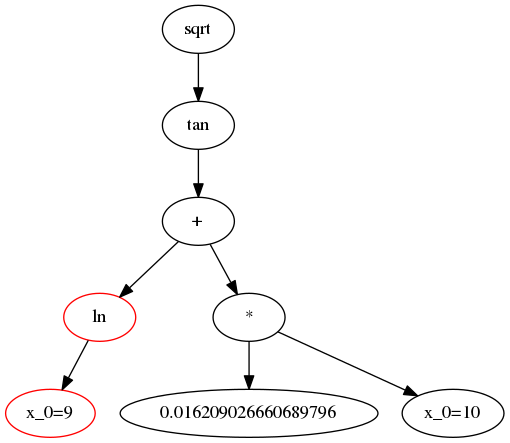
\includegraphics[width=0.8\linewidth]{figures/rightafter.png}
        \caption{B after crossover.}
    \end{subfigure}
    \caption{Symmetric crossover with two random trees.}
    \label{fig:crossover}
\end{figure}

\subsubsection{Mutation}
Mutation works by replacing a randomly chosen subexpression with a newly generated expression. In our implementation this means selecting a node in the tree and replacing it with a new subtree. Our mutation operator can be configured to replace the subtree with one of equal depth or a randomly chosen depth. The insertion point can be made depth-sensitive. A shallow node, a node with a low depth, is the root of a subtree with significant depth. Replacing such a subtree is therefore more likely to have a significant effect on the fitness value. Replacing a deep node will have on average a smaller effect.
The mutation operator is applied either selectively using a cooling schedule, or on the entire population.
The cooling schedule uses the current fitness and the current generation of a tree to decide if the tree is likely to benefit from mutation. This is similar to the approach in simulated annealing \citep{SA}.
Mutation introduces new information into the optimization process (a new subtree). This process can be constructive (lowering fitness) or destructive (increasing fitness). The idea behind the cooling schedule is that for fitter trees the mutation operation will not be able to improve fitness (decrease it), while for less fit trees it has a higher probability to do so.
This probability is estimated using the current generation and fitness value (relative to the population), and using this information a biased random choice is made whether or not to apply mutation. In the experiments in section \ref{secexperiments} we will investigate if this assumption holds, and if it leads to gains in fitness and or effectiveness.
The mutation operator has to generate new subtrees, and therefore the same issues seen in the initialization process which we discussed in section \ref{subsubinvalidexpressions} apply here as well. The mutation operator will generate subtrees until a valid one is found. If the depth sensitive operation proves to generate equal or better fitness values, this could significantly reduce the computation cost of the operator.

\subsubsection{Crossover}
Crossover operates on 2 trees in the population. It selects subtrees from both, and swaps them between each other. The resulting set of 4 trees is scored and the 2 fittest replace the original trees. As with mutation crossover can be configured to operate on a set depth, or select a random depth. It can also work symmetric, picking an equal depth insertion point in both trees.
Crossover in our implementation can be applied in sequence to the entire population, with pairwise mating in order of fitness. Alternatively a random selection can be used. A variant of both, alternating between the two schedules based on a random choice is a third option. This is similar to the roulette wheel selection method, although without replacement.
Crossover, unlike mutation, does not introduce new information in the sense that no new subtrees are generated.
Crossover can be configured to work with a decreasing depth, operating only on deeper nodes at the later stages of the algorithm. The assumption for this mode of operation is similar to that made for mutation.
In Figure \ref{fig:crossoverselection} we see both selection procedures visualized. An important difference with tournament selection is that there is no replacement used in our selection. Crossover will be applied to an expression exactly once.
Crossover is based on the idea that 2 expressions can improve by combining parts of themselves. The operator is selecting these subexpressions randomly. Suppose we have 2 trees, A and B, with randomly selected subtrees a and b respectively. We do not know how much of the fitness of A is the result of its subtree a, and vice versa for B and b. In addition, we do not know or even are able to estimate if a will improve B's fitness value if we replace b with it. In Figure \ref{fig:crossover} we see this visualized for two random trees.
If the expression represented by a tree is a set of separable functions we could use crossover and mutation only on those subexpressions. Unfortunately the search space is composed of both separable and non separable functions, and we do not know in advance if we gain from focussing only on separable solutions. Both crossover and mutation lack this information when dealing with subtrees and are forced to operate as random selectors.

\subsection{Selection}
After evolution a decision has to be made on which expressions to retain in the population. In our tool the population size is fixed, so a replacement is in order. We use an elitist approach. If an expression has a lower (better) fitness value after mutation, it is replaced.
In crossover we combine two expressions r, and t, resulting in two offspring s, u.
From these four expressions the two with minimal fitness survive to the next generation.

\subsection{Archiving}
The algorithm holds an archive that functions as memory for best solutions obtained from the best expressions at the end of a phase., from seeding, or from other processes.
At the end of a phase we archive the j best expressions. J is a parameter ranging from 1 to the population size n. With j == n we risk premature convergence, with j == 1 the risks exists that we lose good expressions from phases which will have to be rediscovered.
While there are numerous archiving strategies described in literature, we use a simple elitist approach. This means that there is no guarantee that the best j samples of phase i are retained, if they have fitness values lower than those present in the archive and the archive has no more empty slots, they will be ignored.
This leads us to the size of the archive. While no exact optimal value for this exists, in order to function as memory between phases it should be at least equal to the amount of phases. The j parameter will influence this choice as well.

\subsection{Representation and data structures}\label{subsectree}
\subsubsection{Expression}
We use a tree representation for an arithmetic expression, where each internal node represent a base function (unary or binary), and each leaf either a feature or a constant.

\paragraph{Tree representation}
We use a hybrid representation of a tree structure. The tree is a set of nodes, where each node holds a list of children nodes. This representation favors recursive traversal algorithms. In addition to this representation, the nodes of a tree are stored in a dictionary keyed on the position of a node. This allows for O(1) access needed by the mutation and crossover operators. The overhead of this extra representation is minimal, since the keys are integers and only a reference is stored. A list representation would be faster in (indexed) access, but would waste memory for sparse trees. With a mix of unary and binary operators the average nodecount of a tree with depth d is $\frac{2^{d+1}-1  + d}{2}$ = O($2^d$) resulting in savings on the order of $2^d$.
The algorithm has the choice which mode of access to use depending on the usage pattern. As an example, selecting a random node in the tree is O(1), selecting a node with a given depth is equally O(1). Splicing subtrees is equally an O(1) operation.

\paragraph{Base functions}
The set of base functions is determined by the problem domain. For symbolic regression we use the following set:\\
+, -, \%, /, max, min, abs, tanh, sin, cos, tan, log, exp, power\\
A problem with this set is the varying domain of each, which may or may not correspond with the domain of the features. A possible extension is to use orthogonal base functions such as Chebyshev polynomials. In our solution the functions listed correspond with their mathematical equivalent, e.g. division by zero is undefined. Other constraints are based on floating point representation (e.g overflow).

\paragraph{Constants}
Constants are fixed values in leaves in the tree. The representation also allows for multiplicative weights for each node, which can be used to further optimize an evolved expression. In contrast to the base functions with a limited set to choose from, constants have the entire floating point range at their disposal. The probability of selecting a 'right' value is extremely small, and domain information is lacking for these constants, it depends on the entire subtree holding the constant. We select a constant from a small range and allow the algorithm to recombine these constants later to larger values. This limiting of the search space can lead to the algorithm converging faster to a suboptimal solution.
The constants are reference objects in the tree, and so can be accessed and modified in place by an optimizer.

\paragraph{Features}
Features are represented as an object holding a reference to a set of input values, and always occur as leaves. The choice for a random leaf is evenly distributed between constants and features.

\subsubsection{Population}
The population of trees is kept in a sorted set, where the key is the fitness value and the value is a reference to the tree representing the expression.  Sorted datastructures are notably lacking from Python, we use the sortedcontainers \cite{sortedcontainers} module which provides sorted datastructures that are designed with performance in mind.
This representation allows for fast access in selecting a (sub)set of fittest trees. It also allows for an O(1) check to see if we already have an equivalent solution, a tree with a fitness score which we already have in the population. This allows our diversity approach mentioned in \ref{subsubdiversity}.
In Figure \ref{fig:uml} we see that the actual data structure used as population is interchangeable. If duplicate fitness values are allowed, and membership testing is no longer needed, a sorted list could be used instead.

\subsection{Parameters}
In this section we briefly list the main parameters of the algorithm and their effects on convergence, runtime and complexity.
\subsubsection{Depth}
The depth of trees can vary between an initial and maximum value. If we know in advance that an optimal solution uses 13 features, the tree should have at least 13 leaves in order to use each feature at least once. This requires a depth of at least 4. In practice the depth will need to be greater due to the use of unary functions, and bloat. Bloat is a known issue in GP \cite{GPBloat}
where the algorithm, unless constrained by limits or an objective function that penalizes depth, will tend to evolve deep trees without gaining much in fitness. In the worst case entire subtrees can be evolved that do not contribute to the fitness value, similar to introns in genetics. These can still have a valid purpose, for example serving as genetic memory. Their disadvantage is clear: a computational overhead without clear effect on the fitness value.
A similar problem arises with the generation of constants. Suppose we would like to generate the constant 3.14, the probability of generating this by a single random call is extremely small. The algorithm will try to build an expression fitting 3.14, for example "1+(3*1) + 28/200". The problem with this is that this process is highly inefficient. It uses iterations that, if a more efficient approach exists, could be used to optimize the fitness value of the tree further. The constant expression wastes nodes that could be used to improve the tree. One approach is folding such expressions into a single constant, which mitigates some of the effects mentioned but does not prevent such subtrees from forming.
Without a solution for this issue, the user would have to take this into account and increase the depth parameter.
From \ref{subsubinvalidexpressions} we know that the initialization process and the mutation operator will become more costly exponential with the increase in depth.
The complexity of our tool is defined by the number of evaluations and the depth of the tree, with the depth having an exponential cost in time and memory.

% complexity
\subsubsection{Population size}
The population size is directly related to convergence rate and the quality of the solution. A very small population will lead to premature convergence, the population is lacking in diversity (or information viewed from a different perspective).
A large population on the other leads to a large increase in runtime, unless the operators only work on a subset of the population. The optimal value is problem specific, but values in the range of [20,50] give a good balance for our implementation.

\subsubsection{Phases and generations}
The execution of the algorithms comprises of g generations and r phases, resulting in a maximum of g x r iterations.
For both parameters a too small value will hinder convergence, while a high value can lead to overfitting. The optimal value is domain specific and dependent on the iterations required to approximate the expected data. This is by virtue of the problem statement unknown. There is a subtle difference between these parameters.
Each phase a reseed of the algorithm is done using the archive. This archive holds the best results from previous phases, external seeds and in a distributed setting the best best solutions from other processes.
The remainder of the population is initialized with a random tree. These trees introduce new information into the optimization process, and while expensive and with a low probability of improving fitness, nonetheless will help avoid premature convergence.
If the archive size is less than the population size, new trees will always be introduced. The rate at which the archive fills is dependent on the number of phases and a parameter which determines how many trees are archived. In a distributed setting this process is accelerated using the input of other processes. If the archive is full after i phases, and the archive size is equal to the population, further phases will no longer have the benefit of newly generated trees. This does not prevent convergence, but could reduce the convergence rate in some scenarios. Increasing g and r both can lead to overfitting, but in order to decide on r we also have to take into account the archiving strategy. In order to find a good starting value for g one can look at the population size.
Diffusion, where the information from each expression is shared with others, will require at least the same amount of generations as there are expressions, depending on the operators and the individual fitness of the expressions. Concentration, where we only look at maximizing the few existing fittest expressions, requires far less generations, but risks premature convergence.
\subsubsection{Samples}
The user can provide the algorithm with input data, or can specify a range from which to sample the input data. In addition, the ratio between training and testing data can be adjusted. Care should be taken in tuning this value. A low ratio will increase the probability that evolved solutions are invalid on the test data, while a high ratio will lead to overfitting.

\subsubsection{Domain}
Domain specific knowledge can significantly reduce the time needed to converge to a solution. In our implementation we assume no domain knowledge. While this increases the complexity of obtaining a good solution, it also makes for a fairer evaluation of the algorithm and optimizations used.

\subsection{Incremental support}\label{subsec:incremental}
Our tool supports incremental operation. The user can provide seeds, expressions that are known or assumed to be good initial approximations. The algorithm writes out the best solutions obtained in an identical format. By combining this the user can create a Design Of Experiment (DOE) setup using the algorithm. As a use case, suppose the user wants to apply symbolic regression on the output of a computationally expensive simulation. The simulator has k features or parameters, each with a different domain and j datapoints. The user wants insights into the correlation of the parameters.
A naive approach would be to generate output data for a full factorial experiment, and feed this into the CSRM tool. For both the simulator and the SR tool the cost of this approach would be prohibitive. It is likely that some features are even irrelevant, leading to unnecessary computation. Instead we can opt for a combined DOE approach. We start with a subset of features k' $<$ k and datapoints j' $<$ j. The simulation results Y' of this subset are then passed to the CSRM algorithm. It generates a set of solutions Q, optimized for this subset of the problem.
The user then adds more parameters, k' $<$ k'' $<$ k and/or datapoints j' $<$ j'' $<$ j, runs the simulator again. The resulting output is given the CSRM tool, with Q as seed. This seed is used as memory of the previous run on the smaller input set. Unless there is no correlation between the incrementing datasets the CSRM tool can use the knowledge gained from the previous run to obtain faster convergence for this new dataset. In addition, by inspecting Q the user can already analyze a (partial) result regarding the initial parameter set.
Suppose k = 5, and only 3 parameters are used in Q. Then the user can exclude the missing two parameters from the remainder of the experiment, as these are unlikely to contribute to the output. With a Latin Hypercube Design DOE approach the design would not have to be reconstructed in order to maintain a space filling design. We will detail this issue further in section \ref{secusecase}.
By chaining the simulator and CSRM tool together in such a way, an efficient DOE approach can potentially save both simulation and regression time, or result in increased quality of solutions.
The advantages are clear :
\begin{itemize}
\item The SR tool can start in parallel with the simulator, instead of having to wait until the simulator has completed all configurations.
\item Intermediary results can be analyzed offering insights into the process that can be acted upon to alter the DOE.
\item The SR tool can reuse previous results as seeds, restricting itself to a relatively small section of the search space instead of starting a blind search.
\end{itemize}
Possible disadvantages are :
\begin{itemize}
\item The SR tool is not guaranteed to return the optimal solution, it is possible the process is misguided by suboptimal solutions. This risk exist as well in the full approach.
\item Interpretation of the results is needed in order to make the decision to prune features or datapoints.
\end{itemize}
We will investigate this approach in our use case in  section \ref{secusecase}.
The diagram \ref{fig:incremental} illustrates a DOE hypercube design using our tool and a simulator. \\
\begin{figure}
\begin{tikzpicture}[node distance=1.5cm, every node/.style={font=\footnotesize}]
\node (start) [startstop] {Start};
\node (featureset) [process, below of=start] {Features};
\node (datapoints) [process, below of=featureset] {Datapoints};
\node (x) [process, right of= datapoints,xshift=4cm, yshift=1.5cm] {X};
\node (simulator) [process, right of=x, xshift=4cm] {Simulator};
\node (srtool) [process, below of=x] {CSRM};
\node (y) [process, below of=simulator] {Y};
\node (expressions) [process, below of=srtool] {Expressions};
\node (analyze) [process, below of=datapoints] {Analyze};

\draw [arrow] (featureset) -- +(+2,0) |-(x) node[near start,sloped,above]{};
\draw [arrow] (start) --(featureset);
\draw [arrow] (datapoints) -- +(+2,0) |-(x) node[near start,sloped,above]{};
\draw [arrow] (x) --node[anchor=south]{input}(simulator);
\draw [arrow] (x) --(srtool);
\draw [arrow] (y) --(srtool);
\draw [arrow] (simulator) --(y);
%\draw [arrow] (simulator) -- +(0,-2) |-(srtool) node[near start,sloped,below]{Y};
%\draw [arrow] (simulator) -- (srtool)node[anchor=east]{Y};
\draw [arrow] (srtool) --node[anchor=east]{}(expressions);
\draw [arrow] (expressions)-- +(-2,0) |- (srtool) node[near start,sloped,below, anchor=south] {seeds};
\draw [arrow] (expressions)-- +(-2, 0) |- (analyze) node[near start,sloped,above, anchor=south] {};
\draw [arrow] (expressions)-- +(-2, 0) |- (analyze) node[near start,sloped,above, anchor=south] {};
\draw [arrow] (analyze)-- +(-2, 0) |- (featureset) node[near start,sloped,above, anchor=south] {};
\draw [arrow] (analyze)-- +(-2, 0) |- (datapoints) node[near start,sloped,above, anchor=south] {reduces/expands};

\end{tikzpicture}
\caption{Incremental DOE using CSRM and a simulator.}
\label{fig:incremental}
\end{figure}

\subsection{Statistics and visualization}
Stochastic algorithms are notoriously hard to debug, analyze and reason about. By virtue of the problem statement we do not know whether the returned solution is what is expected. The size of the search space makes detecting all edge cases infeasible. In addition the algorithm functions as a black box, where output is presented to the user without a clear trace indicating how or why this output was obtained. For both developer and practitioner insight into the algorithms inner workings is vital.
Our tool provides a wealth of runtime statistics ranging from fitness values per expression for each point in the execution, convergence behavior over time, depth and complexity of the expressions, cost of evaluations, effectiveness of operators, correlation between training and test fitness values and more. These statistics can be saved to disk for later analysis, or displayed in plots in a browser. Using this information the user can tune the parameters of the algorithm, for example reducing the number of phases when overfitting is detected. The developer can look at how effective modifications are to the operators, archiving strategy and so on.
It is even possible to trace the entire run of the algorithm step by step by saving the expressions in tree form, displayed in an SVG image rendered by Graphviz \cite{graphviz}. In Figure \ref{fig:viz} a selection of the collected statistics on a testfunction is shown. The third of our set of testproblems was used with a depth $\in$ [4,10], 30 generations, populationsize 30, and 4 phases.
 \begin{figure}
    \centering
    \begin{subfigure}{0.5\textwidth}
    \centering
        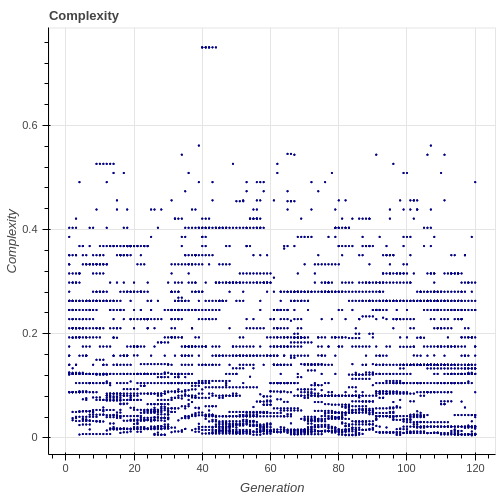
\includegraphics[width=0.8\linewidth]{figures/viz_complexity.png}
        \caption{Scaled complexity over generations.}
    \end{subfigure}%
    \begin{subfigure}{0.5\textwidth}
    \centering
        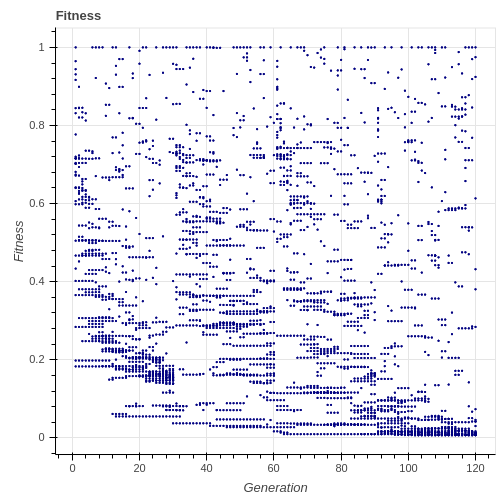
\includegraphics[width=0.8\linewidth]{figures/viz_fitness.png}
        \caption{Fitness values over generations.}
    \end{subfigure}
        \begin{subfigure}{0.5\textwidth}
    \centering
        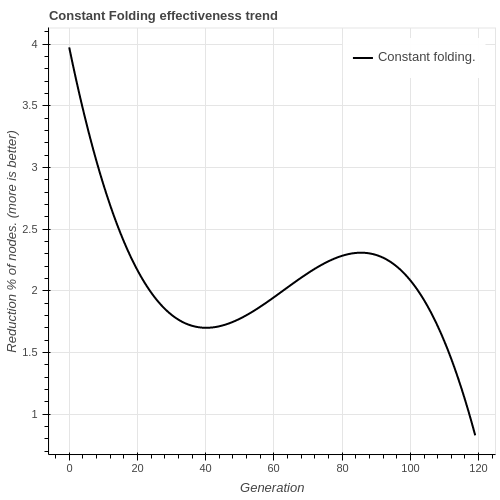
\includegraphics[width=0.8\linewidth]{figures/viz_constantfoldingtrend.png}
        \caption{Constant folding savings.}
    \end{subfigure}%
    \begin{subfigure}{0.5\textwidth}
    \centering
        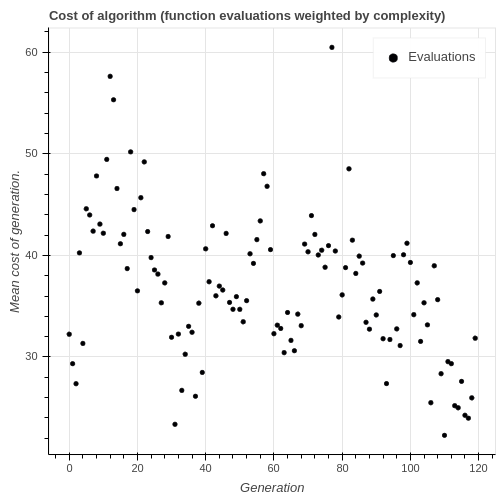
\includegraphics[width=0.8\linewidth]{figures/viz_meancost.png}
        \caption{Mean evaluation cost.}
    \end{subfigure}
        \begin{subfigure}{0.5\textwidth}
    \centering
        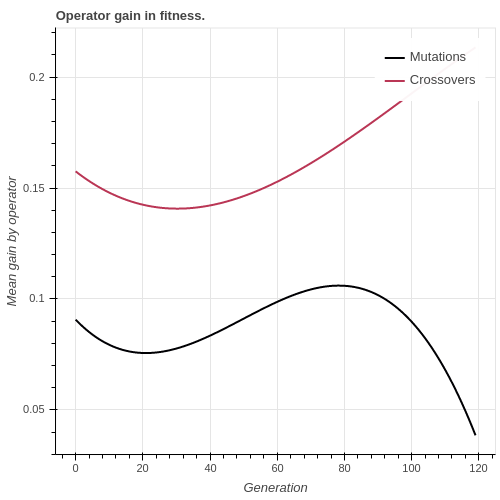
\includegraphics[width=0.8\linewidth]{figures/viz_operatorgaintrend.png}
        \caption{Operator gain.}
    \end{subfigure}%
    \begin{subfigure}{0.5\textwidth}
    \centering
        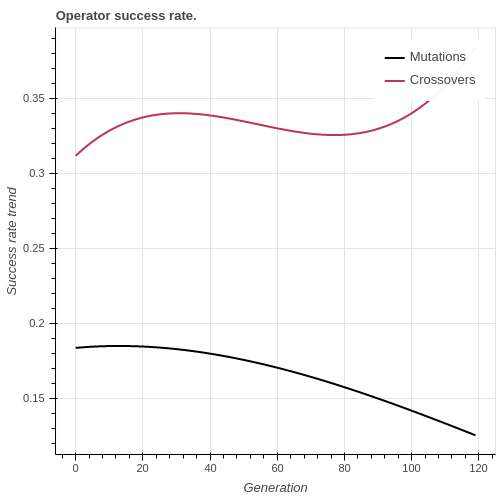
\includegraphics[width=0.8\linewidth]{figures/viz_operatorsuccessratetrend.png}
        \caption{Operator success rate.}
    \end{subfigure}
    \caption{Selection of visualizations generated by CSRM.}
    \label{fig:viz}
\end{figure}

%\subsection{Conclusion}
%In this section we have covered in detail the design of the CSRM tool, highlighting the choices made. We have enumerated the features
%% Full featured tool offers insight, variation, testing.
%
